\documentclass[final]{beamer} 
\mode<presentation>
\usepackage{inconsolata}
\renewcommand*\familydefault{\ttdefault}
\usepackage{dejavu}
\renewcommand*\familydefault{\sfdefault}
\usepackage{lmodern}
\renewcommand\mathfamilydefault{\rmdefault}

\usepackage[T1]{fontenc}
\usepackage{listings}
\lstset{language=Haskell,basicstyle=\ttfamily,xleftmargin=5mm}
\usepackage{verbatim}
\usepackage{tikz}
\usetikzlibrary{arrows, fit, shapes}
\setbeamertemplate{frametitle}{
  \begin{beamercolorbox}[wd=0.95\paperwidth]{lower separation line head}
  \hspace{0.5cm}
  \insertframetitle
  \hfill
  \includegraphics[width=.15\linewidth]{unm}
  \end{beamercolorbox}
}

\setbeamertemplate{footline}{}

\mode<all>

\definecolor{red}{RGB}{205,16,65}
\definecolor{grey}{RGB}{109,111,113}

\setbeamerfont{structure}{family=\sffamily}
\setbeamercolor{structure}{fg=red}
\setbeamerfont{normal text}{family=\sffamily}
\setbeamercolor{normal text}{fg=grey,bg=white}

\title{Subtypes for Free!}
\author{George Stelle}
\institute{University of New Mexico}
%\date{\today} 

\begin{document}
\begin{frame}[fragile]
\titlepage
\end{frame}
\begin{frame}{Types}
\centering
\onslide<1->{Why types?} \\
\vspace{2cm} 
\onslide<2->{\emph{So evaluation can't go wrong at runtime}} \\
\vspace{2cm}
\onslide<3->{\texttt{head :: List a -> a}} \\
\onslide<4->{\texttt{tail :: List a -> List a}} \\
\onslide<5->{\texttt{fromJust :: Maybe a -> a}}
\end{frame}

\begin{frame}[fragile]{Our Solution}
\centering
\onslide<1->{Subtypes from Parametric Polymorphism} \\
\onslide<2->{+ \\ Scott Encodings of ADTs} \\
\vspace{1cm}
\onslide<3->{(Also unification)}

\end{frame}

\begin{frame}[fragile]{Subtypes from Parametric Polymorphism}

\centering
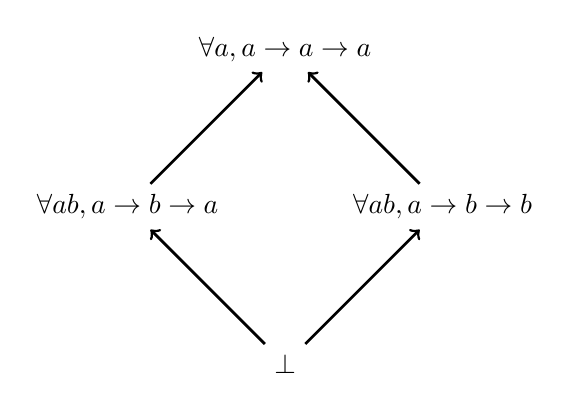
\begin{tikzpicture}[->, line width=1pt, auto, node distance=4cm]
\node (1) at (2,4) {$\forall a, a \rightarrow a \rightarrow a$};
\node (2) at (0,2) {$\forall a b, a \rightarrow b \rightarrow a$};
\node (3) at (4,2) {$\forall a b, a \rightarrow b \rightarrow b$};
\node (4) at (2,0) {$\bot$};

\path (2) edge node {} (1)
      (3) edge node {} (1)
      (4) edge node {} (2)
      (4) edge node {} (3);
\end{tikzpicture}

\end{frame}

\begin{frame}[fragile]{+ Scott Encodings of \texttt{Bool}}

\centering
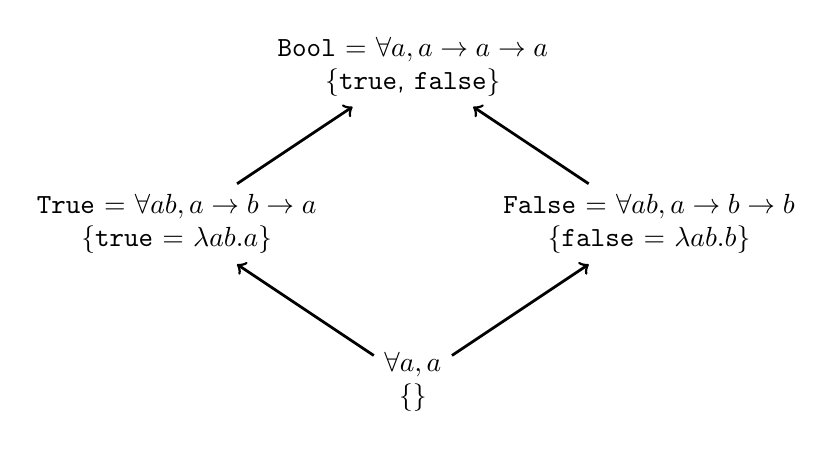
\begin{tikzpicture}[->, align=center,line width=1pt, auto, node distance=4cm]
\node (1) at (2,4) {\texttt{Bool} = $\forall a, a \rightarrow a \rightarrow a$
\\ \{\texttt{true}, \texttt{false}\}};
\node (2) at (-1,2) {\texttt{True} = $\forall a b, a \rightarrow b \rightarrow
a$ \\ \{\texttt{true} = $\lambda a b. a$\} };
\node (3) at (5,2) {\texttt{False} = $\forall a b, a \rightarrow b \rightarrow
b$ \\ \{\texttt{false} = $\lambda a b. b$\} };
\node (4) at (2,0) {$\forall a, a$ \\ \{\}};

\path (2) edge node {} (1)
      (3) edge node {} (1)
      (4) edge node {} (2)
      (4) edge node {} (3);
\end{tikzpicture}

\end{frame}

\begin{frame}[fragile]{\texttt{Maybe}}

\begin{center}
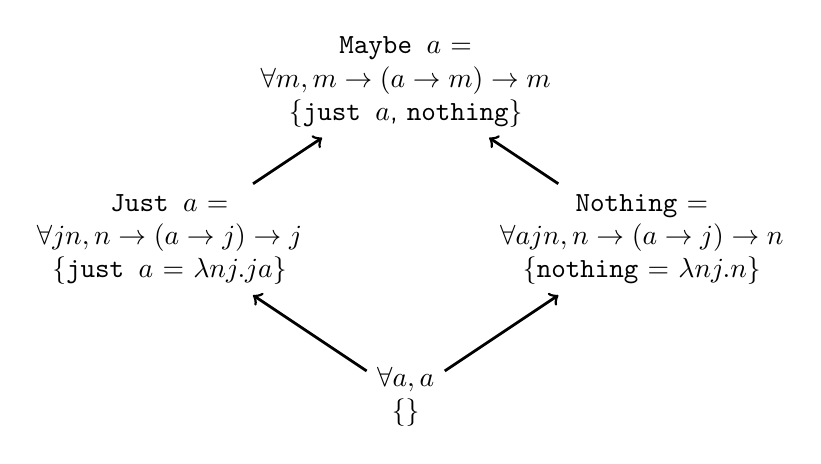
\begin{tikzpicture}[->, align=center, line width=1pt, auto, node distance=4cm]
\node (1) at (2,4) {\texttt{Maybe $a$} = \\ $\forall m, m \rightarrow (a
\rightarrow m) \rightarrow m$ \\ \{\texttt{just $a$}, \texttt{nothing}\}};
\node (2) at (-1,2) {\texttt{Just $a$} = \\ $\forall j n, n \rightarrow (a \rightarrow
j) \rightarrow j$ \\ \{\texttt{just $a$} = $\lambda n j. j a$\} };
\node (3) at (5,2) {\texttt{Nothing} = \\ $\forall a j n, n \rightarrow (a
\rightarrow j) \rightarrow n$ \\ \{\texttt{nothing} = $\lambda n j.n$\} };
\node (4) at (2,0) {$\forall a, a$ \\ \{\} };

\path (2) edge node {} (1)
      (3) edge node {} (1)
      (4) edge node {} (2)
      (4) edge node {} (3);
\end{tikzpicture}
\end{center}
\onslide<2->{\texttt{fromJust :: Just a -> a}} \\ 
\onslide<3->{\texttt{fromJust j = j (undefined :: Void) id}}

\end{frame}

\begin{frame}[fragile]{Other Examples}

\onslide<1->{\texttt{head :: Cons a -> a}} \\
\onslide<1->{\texttt{tail :: Cons a -> List a}} \\
\onslide<2->{\texttt{eval :: Expr -> Value}} \\
\onslide<3->{\texttt{warrior :: DaggerOrSword -> Warrior}}
\vspace{1cm}

\onslide<4->{\texttt{true `and` false :: False}} \\
\onslide<5->{\texttt{null nil :: True}}

\end{frame}

\begin{frame}[fragile]{Drawbacks and Limitations}
\begin{itemize}
\item <1-> Impredicative types, e.g. \texttt{List (List Bool)}
\item <2-> Type classes, e.g. \texttt{Show Bool}
\item <3-> Recursive types, e.g. (!!)
\item <4-> Performance
\item <5-> Verbose
\item <6-> Meet, e.g. \texttt{not :: Bool -> Bool}
\end{itemize}
\end{frame}

\begin{comment}

\begin{frame}[fragile]{Related work}

\centering
\begin{tikzpicture}[-, line width=1pt, auto, node distance=4cm]
%\node (5) at (0,6) {\emph{More Expressive Power}};
\node (4) at (0,5) {Dependent Types};
\node (3) at (0,4) {Refinement Types};
\node (2) at (0,3 {GADTs / Phantom Types};
\node (1) at (0,2) {\color{red} Free Subtypes};
\node (0) at (0,1) {Haskell98};
%\node (6) at (0,0) {\emph{Easier to Use}};

\path (0) edge node {} (1)
      (1) edge node {} (2)
      (2) edge node {} (3)
      (3) edge node {} (4);
\end{tikzpicture}
\end{frame}
\end{comment}

\begin{frame}

\centering

Thanks!

\vspace{1cm}

Questions?

\end{frame}

\end{document}
